% answers.tex —— 2011 年·湖南卷·文科 · 参考答案与详细解析片段
% 由 tools/generate_projects.py 依来源总账自 2011/2011_数学真题_湖南文_试题.md + 2011/2011_数学真题_湖南文_解析正文.md + 2011/2011_数学真题_湖南文_答案要点.md 生成，勿手改（改源 MD 后重跑）

\begin{answer}
\gksolhead{1}{}

\textbf{题目}：

设全集 $U=M\cup N=\{1,2,3,4,5\}$，$M\cap\complement_UN=\{2,4\}$，则 $N=$\mbox{（　　）}

（A）$\{1,2,3\}$

（B）$\{1,3,5\}$

（C）$\{1,4,5\}$

（D）$\{2,3,4\}$

\Needspace{4\baselineskip}
\textbf{解析}
$\complement_UN$ 是 $U$ 中不属于 $N$ 的元素。$M\cap\complement_UN=\{2,4\}$，故 $2,4\in M$ 且 $2,4\notin N$；又 $U=M\cup N$，不在 $M$ 中的 $1,3,5$ 必在 $N$ 中。故 $N=\{1,3,5\}$。选 B。

\gkanswer{答案：B。}

\end{answer}
\begin{answer}
\gksolhead{2}{}

\textbf{题目}：

若 $a$，$b\in\mathbf R$，$\mathrm i$ 为虚数单位，且 $(a+\mathrm i)\mathrm i=b+\mathrm i$，则\mbox{（　　）}

（A）$a=1$，$b=1$

（B）$a=-1$，$b=1$

（C）$a=1$，$b=-1$

（D）$a=-1$，$b=-1$

\Needspace{4\baselineskip}
\textbf{解析}
$(a+\mathrm i)\mathrm i=-1+a\mathrm i=b+\mathrm i$，故 $a=1$，$b=-1$。选 C。

\gkanswer{答案：C。}

\end{answer}
\begin{answer}
\gksolhead{3}{}

\textbf{题目}：

“$x>1$”是“$|x|>1$”的\mbox{（　　）}

（A）充分不必要条件

（B）必要不充分条件

（C）充分必要条件

（D）既不充分又不必要条件

\Needspace{4\baselineskip}
\textbf{解析}
$x>1\Rightarrow|x|>1$；反之 $x<-1$ 时 $|x|>1$ 但 $x>1$ 不成立。故充分不必要。选 A。

\gkanswer{答案：A。}

\end{answer}
\begin{answer}
\gksolhead{4}{}

\textbf{题目}：

如图是某几何体的三视图，则该几何体的体积为\mbox{（　　）}

（A）$9\pi+42$

（B）$36\pi+18$

（C）$\frac92\pi+12$

（D）$\frac92\pi+18$
\nopagebreak[4]
\begin{center}% 2011 年湖南卷理科第 3 题：三视图（圆柱与长方体组合）。
% 来源 PDF：普通高考/2011/2011湖南理.pdf，SHA-256 09b67f1db8e6a280165cf8431211a968163c0d0f262a50068dd607607a9ec578。
% 原页：第 1 页第 1 栏，书页码 671。示意图。
\begin{tikzpicture}[>=stealth, semithick, font=\small, scale=0.85]
  \draw[thick] (0,0) rectangle (2.4,1.6);
  \node[below] at (1.2,-0.1) {正视图};
  \draw[thick] (3.0,0) rectangle (4.6,1.6);
  \node[below] at (3.8,-0.1) {侧视图};
  \draw[thick] (1.2,-2.6) circle (0.8);
  \draw[thick] (0.4,-2.6)--(2.0,-2.6);
  \node[below] at (1.2,-3.5) {俯视图};
\end{tikzpicture}
\end{center}
\nopagebreak[4]
\Needspace{4\baselineskip}
\textbf{解析}
\Needspace{5\baselineskip}
几何体为圆柱（底面直径 $3$、高 $2$）与长方体（$3\times2\times2$）的组合，体积
\nopagebreak[4]
\[\pi\left(\frac32\right)^2\cdot2+12=\frac92\pi+12.\]
选 C。

\gkanswer{答案：C。}

\end{answer}
\begin{answer}
\gksolhead{5}{}

\textbf{题目}：

通过随机询问 $110$ 名性别不同的大学生是否爱好某项运动，得到列联表（同理科第 4 题），算得 $K^2\approx7.8$。参照附表，得到的正确结论是\mbox{（　　）}

（A）有 $99\%$ 以上的把握认为“爱好该项运动与性别有关”

（B）有 $99\%$ 以上的把握认为“爱好该项运动与性别无关”

（C）在犯错误的概率不超过 $0.1\%$ 的前提下，认为“爱好该项运动与性别有关”

（D）在犯错误的概率不超过 $0.1\%$ 的前提下，认为“爱好该项运动与性别无关”

\Needspace{4\baselineskip}
\textbf{解析}
$K^2\approx7.8>6.635$，对应 $P=0.010$，故有 $99\%$ 以上把握认为有关。选 A。

\gkanswer{答案：A。}

\end{answer}
\begin{answer}
\gksolhead{6}{}

\textbf{题目}：

设双曲线 $\dfrac{x^2}{a^2}-\dfrac{y^2}9=1$（$a>0$）的渐近线方程为 $3x\pm2y=0$，则 $a$ 的值为\mbox{（　　）}

（A）$4$

（B）$3$

（C）$2$

（D）$1$

\Needspace{4\baselineskip}
\textbf{解析}
渐近线 $y=\pm\dfrac3a x$，与 $y=\pm\dfrac32x$ 比较得 $a=2$。选 C。

\gkanswer{答案：C。}

\end{answer}
\begin{answer}
\gksolhead{7}{}

\textbf{题目}：

曲线 $y=\dfrac{\sin x}{\sin x+\cos x}-\dfrac12$ 在点 $M\left(\dfrac\pi4,0\right)$ 处的切线的斜率为\mbox{（　　）}

（A）$-\frac12$

（B）$\frac12$

（C）$-\frac{\sqrt2}2$

（D）$\frac{\sqrt2}2$

\Needspace{4\baselineskip}
\textbf{解析}
\nopagebreak[4]
\[y'=\frac{\cos x(\sin x+\cos x)-\sin x(\cos x-\sin x)}{(\sin x+\cos x)^2}
=\frac{1}{(\sin x+\cos x)^2}.\]
在 $x=\dfrac\pi4$ 处 $\sin x+\cos x=\sqrt2$，故斜率为 $\dfrac12$。选 B。

\gkanswer{答案：B。}

\end{answer}
\begin{answer}
\gksolhead{8}{}

\textbf{题目}：

已知函数 $f(x)=\mathrm e^x-1$，$g(x)=-x^2+4x-3$，若有 $f(a)=g(b)$，则 $b$ 的取值范围为\mbox{（　　）}

（A）$[2-\sqrt2,2+\sqrt2]$

（B）$(2-\sqrt2,2+\sqrt2)$

（C）$[1,3]$

（D）$(1,3)$

\Needspace{4\baselineskip}
\textbf{解析}
\Needspace{5\baselineskip}
$f(x)=\mathrm e^x-1>-1$，故 $g(b)>-1$：
\nopagebreak[4]
\[-b^2+4b-3>-1\Longrightarrow b^2-4b+2<0\Longrightarrow2-\sqrt2<b<2+\sqrt2.\]
选 B。

\gkanswer{答案：B。}

\end{answer}
\begin{answer}
\gksolhead{9}{}

\textbf{题目}：

在直角坐标系 $xOy$ 中，曲线 $C_1$ 的参数方程为 $\begin{cases}x=2\cos\alpha,\\y=\sqrt3\sin\alpha\end{cases}$（$\alpha$ 为参数），在极坐标系中曲线 $C_2$ 的方程为 $\rho(\cos\theta-\sin\theta)+1=0$，则 $C_1$ 与 $C_2$ 的交点个数为 $\underline{\qquad}$。

\Needspace{4\baselineskip}
\textbf{解析}
$C_1:\dfrac{x^2}4+\dfrac{y^2}3=1$；$C_2:x-y+1=0$。中心到直线距离 $\dfrac1{\sqrt2}<1$，直线与椭圆相交于 $2$ 点。

\gkanswer{答案：$2$。}

\end{answer}
\begin{answer}
\gksolhead{10}{}

\textbf{题目}：

已知某试验范围为 $[10,90]$，若用分数法进行 $4$ 次优选试验，则第二次试点可以是 $\underline{\qquad}$。

\Needspace{4\baselineskip}
\textbf{解析}
分数法 $4$ 次试验取分数 $\dfrac58$。第一次试点 $10+80\times\dfrac58=60$，第二次试点 $10+80\times\dfrac38=40$（或第一次取 $40$、第二次取 $60$）。填 $40$。

\gkanswer{答案：$40$。}

\end{answer}
\begin{answer}
\gksolhead{11}{}

\textbf{题目}：

若执行如图所示的框图，输入 $x_1=1$，$x_2=2$，$x_3=4$，$x_4=8$，则输出的数等于 $\underline{\qquad}$。
\nopagebreak[4]
\begin{center}% 2011 年湖南卷文科第 11 题：程序框图（求四个数的平均数）。
% 来源 PDF：普通高考/2011/2011湖南文.pdf，SHA-256 0982cbf095a3c71ebb0e1c16297a96391db09ef14484f81a1130924443ea395d。
% 原页：第 1 页第 2 栏中部，书页码 673。
\begin{tikzpicture}[>=stealth, semithick, font=\small]
  \node[draw, rounded corners=0.12cm, minimum width=1.2cm, minimum height=0.5cm] (start) at (0,0) {开始};
  \node[draw, minimum width=3.4cm, minimum height=0.55cm] (in) at (0,-1.2) {输入 $x_1,x_2,x_3,x_4$};
  \node[draw, minimum width=2.4cm, minimum height=0.5cm] (init) at (0,-2.4) {$i=1,\ x=0$};
  \node[draw, minimum width=2.6cm, minimum height=0.55cm] (add) at (0,-3.7) {$x=x+x_i$};
  \node[draw, minimum width=1.6cm, minimum height=0.5cm] (inc) at (2.9,-3.7) {$i=i+1$};
  \node[draw, diamond, aspect=1.7, minimum width=1.4cm, minimum height=0.9cm] (test) at (0,-5.1) {$i<4$};
  \node[draw, minimum width=2.0cm, minimum height=0.5cm] (div) at (0,-6.4) {$x=\dfrac x4$};
  \node[draw, trapezium, trapezium left angle=72, trapezium right angle=108,
        minimum width=1.6cm, minimum height=0.55cm] (out) at (0,-7.6) {输出 $x$};
  \node[draw, rounded corners=0.12cm, minimum width=1.2cm, minimum height=0.5cm] (stop) at (0,-8.7) {结束};
  \draw[->] (start)--(in); \draw[->] (in)--(init); \draw[->] (init)--(add); \draw[->] (add)--(test);
  \draw[->] (test.east) -| (inc.north) node[pos=0.25, above] {是};
  \draw[->] (inc.south) |- (add.east);
  \draw[->] (test.south)--(div.north) node[midway, right] {否};
  \draw[->] (div)--(out); \draw[->] (out)--(stop);
\end{tikzpicture}
\end{center}
\nopagebreak[4]
\Needspace{4\baselineskip}
\textbf{解析}
\Needspace{5\baselineskip}
框图求四个输入的平均数：
\nopagebreak[4]
\[\frac{1+2+4+8}4=\frac{15}4.\]

\gkanswer{答案：$\dfrac{15}4$。}

\end{answer}
\begin{answer}
\gksolhead{12}{}

\textbf{题目}：

已知 $f(x)$ 为奇函数，$g(x)=f(x)+9$，$g(-2)=3$，则 $f(2)=$ $\underline{\qquad}$。

\Needspace{4\baselineskip}
\textbf{解析}
$g(-2)=f(-2)+9=3$，故 $f(-2)=-6$；$f$ 为奇函数，$f(2)=6$。

\gkanswer{答案：$6$。}

\end{answer}
\begin{answer}
\gksolhead{13}{}

\textbf{题目}：

设向量 $\boldsymbol a$，$\boldsymbol b$ 满足 $|\boldsymbol a|=2\sqrt5$，$\boldsymbol b=(2,1)$，且 $\boldsymbol a$ 与 $\boldsymbol b$ 的方向相反，则 $\boldsymbol a$ 的坐标为 $\underline{\qquad}$。

\Needspace{4\baselineskip}
\textbf{解析}
\Needspace{5\baselineskip}
$\boldsymbol b=(2,1)$，$|\boldsymbol b|=\sqrt5$。$\boldsymbol a$ 与 $\boldsymbol b$ 反向，且 $|\boldsymbol a|=2|\boldsymbol b|$，故
\nopagebreak[4]
\[\boldsymbol a=-2\boldsymbol b=(-4,-2).\]

\gkanswer{答案：$(-4,-2)$。}

\end{answer}
\begin{answer}
\gksolhead{14}{}

\textbf{题目}：

设 $m>1$，在约束条件 $\begin{cases}y\geqslant x,\\y\leqslant mx,\\x+y\leqslant1\end{cases}$ 下，目标函数 $z=x+5y$ 的最大值为 $4$，则 $m$ 的值为 $\underline{\qquad}$。

\Needspace{4\baselineskip}
\textbf{解析}
\Needspace{5\baselineskip}
目标函数在 $\left(\dfrac1{m+1},\dfrac m{m+1}\right)$ 取最大值：
\nopagebreak[4]
\[z_{\max}=\frac{1+5m}{m+1}=4\Longrightarrow1+5m=4m+4\Longrightarrow m=3.\]

\gkanswer{答案：$3$。}

\end{answer}
\begin{answer}
\gksolhead{15}{}

\textbf{题目}：

已知圆 $C:x^2+y^2=12$，直线 $l:4x+3y=25$。

（1） 圆 $C$ 的圆心到直线 $l$ 的距离为 $\underline{\qquad}$；

（2） 圆 $C$ 上任意一点 $A$ 到直线 $l$ 的距离小于 $2$ 的概率为 $\underline{\qquad}$。

\Needspace{4\baselineskip}
\textbf{解析}
\gksubpart{(1)}
圆心到直线距离 $\dfrac{25}{\sqrt{4^2+3^2}}=5$。

\gksubpart{(2)}
\Needspace{5\baselineskip}
圆半径 $2\sqrt3$。圆上点到直线距离
\nopagebreak[4]
\[d=\frac{|4x+3y-25|}5=\left|2\sqrt3\sin(\theta+\varphi)-5\right|.\]
$d<2$ 等价于 $3<2\sqrt3\sin(\theta+\varphi)<7$，即 $\sin(\theta+\varphi)>\dfrac{\sqrt3}2$，对应圆心角 $\dfrac\pi3$，概率 $\dfrac{\pi/3}{2\pi}=\dfrac16$。

\gkanswer{答案（1）：$5$。}

\gkanswer{答案（2）：$\dfrac16$。}

\end{answer}
\begin{answer}
\gksolhead{16}{}

\textbf{题目}：

给定 $k\in\mathbf N^*$，设函数 $f:\mathbf N^*\to\mathbf N^*$ 满足：对于任意大于 $k$ 的正整数 $n$，$f(n)=n-k$。

（1） 设 $k=1$，则其中一个函数 $f$ 在 $n=1$ 处的函数值为 $\underline{\qquad}$；

（2） 设 $k=4$，且当 $n\leqslant4$ 时，$2\leqslant f(n)\leqslant3$，则不同的函数 $f$ 的个数为 $\underline{\qquad}$。

\Needspace{4\baselineskip}
\textbf{解析}
\gksubpart{(1)}
$k=1$ 时 $n>1$ 有 $f(n)=n-1$，$f(1)$ 可任取正整数，例如 $1$。

\gksubpart{(2)}
$k=4$ 时，$n=1,2,3,4$ 的函数值各有 $2$ 种选择（$2$ 或 $3$），共 $2^4=16$ 个不同函数。

\gkanswer{答案（1）：$1$。}

\gkanswer{答案（2）：$16$。}

\end{answer}
\begin{answer}
\gksolhead{17}{}

\textbf{题目}：

在 $\triangle ABC$ 中，角 $A$，$B$，$C$ 所对的边分别为 $a$，$b$，$c$，且满足 $c\sin A=a\cos C$。

（1） 求角 $C$ 的大小；

（2） 求 $\sqrt3\sin A-\cos\left(B+\dfrac\pi4\right)$ 的最大值，并求取得最大值时角 $A$，$B$ 的大小。

\Needspace{4\baselineskip}
\textbf{解析}
\gksubpart{(1)}
由正弦定理 $c\sin A=a\sin C$，条件化为 $a\sin C=a\cos C$，故 $\tan C=1$，$C=\dfrac\pi4$。

\gksubpart{(2)}
\Needspace{5\baselineskip}
$B=\dfrac{3\pi}4-A$，$B+\dfrac\pi4=\pi-A$，故
\nopagebreak[4]
\[\sqrt3\sin A-\cos\left(B+\frac\pi4\right)=\sqrt3\sin A+\cos A=2\sin\left(A+\frac\pi6\right).\]
最大值为 $2$，当 $A+\dfrac\pi6=\dfrac\pi2$ 即 $A=\dfrac\pi3$、$B=\dfrac{5\pi}{12}$。

\gkanswer{答案（1）：$C=\dfrac\pi4$。}

\gkanswer{答案（2）：最大值 $2$，此时 $A=\dfrac\pi3$，$B=\dfrac{5\pi}{12}$。}

\end{answer}
\begin{answer}
\gksolhead{18}{}

\textbf{题目}：

\Needspace{5\baselineskip}
某河流上的一座水力发电站，每年六月份的发电量 $Y$（单位：万千瓦时）与该河上游在六月份的降雨量 $X$（单位：毫米）有关。据统计，当 $X=70$ 时，$Y=460$；$X$ 每增加 $10$，$Y$ 增加 $5$。已知近 $20$ 年 $X$ 的值为
\nopagebreak[4]
\[140,110,160,70,200,160,140,160,220,200,110,160,160,200,140,110,160,220,140,160.\]

（1） 完成频率分布表（降雨量 $70,110,140,160,200,220$ 对应频率）；

（2） 假定今年六月份的降雨量与近 $20$ 年分布规律相同，并将频率视为概率，求今年六月份该水力发电站的发电量低于 $490$ 或超过 $530$ 的概率。

\Needspace{4\baselineskip}
\textbf{解析}
\gksubpart{(1)}
\Needspace{5\baselineskip}
统计得 $70,110,140,160,200,220$ 的频数分别为 $1,3,4,7,3,2$，频率依次为
\nopagebreak[4]
\[\frac1{20},\ \frac3{20},\ \frac4{20},\ \frac7{20},\ \frac3{20},\ \frac2{20}.\]

\gksubpart{(2)}
\Needspace{5\baselineskip}
$Y=460+\dfrac{X-70}{2}$。$Y<490\iff X<130$，对应 $70,110$，概率 $\dfrac4{20}$；$Y>530\iff X>210$，对应 $220$，概率 $\dfrac2{20}$。故
\nopagebreak[4]
\[P=\frac4{20}+\frac2{20}=\frac3{10}.\]

\gkanswer{答案（1）：频率依次为 $\dfrac1{20},\dfrac3{20},\dfrac4{20},\dfrac7{20},\dfrac3{20},\dfrac2{20}$。}

\gkanswer{答案（2）：$\dfrac3{10}$。}

\end{answer}
\begin{answer}
\gksolhead{19}{}

\textbf{题目}：

如图，在圆锥 $PO$ 中，已知 $PO=\sqrt2$，$\odot O$ 的直径 $AB=2$，点 $C$ 在 $\overset{\frown}{AB}$ 上，且 $\angle CAB=30^\circ$，$D$ 为 $AC$ 的中点。

（1） 证明：$AC\perp$ 平面 $POD$；

（2） 求直线 $OC$ 和平面 $PAC$ 所成角的正弦值。
\nopagebreak[4]
\begin{center}% 2011 年湖南卷文科第 19 题：圆锥 PO，C 在弧 AB 上且 ∠CAB=30°，D 为 AC 中点。
% 来源 PDF：普通高考/2011/2011湖南文.pdf，SHA-256 0982cbf095a3c71ebb0e1c16297a96391db09ef14484f81a1130924443ea395d。
% 原页：第 2 页第 1 栏下部，书页码 674。示意。
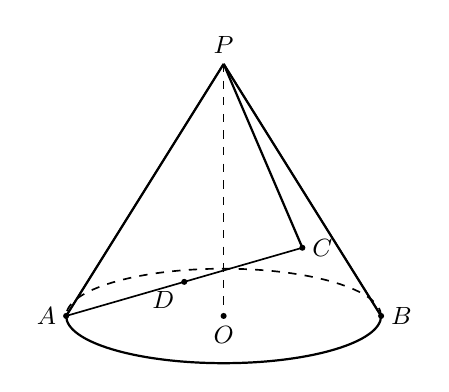
\begin{tikzpicture}[>=stealth, semithick, font=\small, scale=1.0]
  \draw[thick] (0,3.2)--(-2,0);
  \draw[thick] (0,3.2)--(2,0);
  \draw[thick] (-2,0) arc (180:360:2 and 0.6);
  \draw[dashed] (2,0) arc (0:180:2 and 0.6);
  \draw[dashed] (0,3.2)--(0,0);
  \coordinate (A) at (-2,0);
  \coordinate (B) at (2,0);
  \coordinate (C) at (1,0.866);
  \coordinate (D) at (-0.5,0.433);
  \draw[thick] (0,3.2)--(C);
  \draw (A)--(C);
  \draw (0,3.2)--(A); \draw (0,3.2)--(B);
  \fill (A) circle (1.1pt) node[left] {$A$};
  \fill (B) circle (1.1pt) node[right] {$B$};
  \fill (C) circle (1.1pt) node[right] {$C$};
  \fill (D) circle (1.1pt) node[below left] {$D$};
  \fill (0,0) circle (1.1pt) node[below] {$O$};
  \node[above] at (0,3.2) {$P$};
\end{tikzpicture}
\end{center}
\nopagebreak[4]
\Needspace{4\baselineskip}
\textbf{解析}
\gksubpart{(1)}
\Needspace{5\baselineskip}
取 $O(0,0,0)$，$A(-1,0,0)$，$B(1,0,0)$，$P(0,0,\sqrt2)$。由 $\angle CAB=30^\circ$ 得 $C\left(\dfrac12,\dfrac{\sqrt3}2,0\right)$，$D$ 为 $AC$ 中点 $\left(-\dfrac14,\dfrac{\sqrt3}4,0\right)$。
\nopagebreak[4]
\[\overrightarrow{AC}=\left(\frac32,\frac{\sqrt3}2,0\right),\qquad \overrightarrow{OD}=\left(-\frac14,\frac{\sqrt3}4,0\right),\]
点积 $-\dfrac38+\dfrac38=0$，故 $AC\perp OD$；又 $AC\perp PO$，故 $AC\perp$ 平面 $POD$。

\gksubpart{(2)}
\Needspace{5\baselineskip}
$\overrightarrow{OC}=\left(\dfrac12,\dfrac{\sqrt3}2,0\right)$。平面 $PAC$ 的法向量
\nopagebreak[4]
\[\boldsymbol n=\overrightarrow{PA}\times\overrightarrow{PC}=(-1,0,-\sqrt2)\times\left(\frac12,\frac{\sqrt3}2,-\sqrt2\right)
=\left(\frac{\sqrt6}2,-\frac{3\sqrt2}2,-\frac{\sqrt3}2\right).\]
\nopagebreak[4]
\[|\cos\langle\overrightarrow{OC},\boldsymbol n\rangle|=\frac{\left|\frac{\sqrt6}4-\frac{3\sqrt6}4\right|}{1\cdot3\sqrt3}
=\frac{\sqrt6/2}{3\sqrt3}=\frac{\sqrt2}{12}.\]
故所求正弦值为 $\dfrac{\sqrt2}{12}$。

\gkanswer{答案（1）：证明见解析。}

\gkanswer{答案（2）：$\dfrac{\sqrt2}{12}$。}

\end{answer}
\begin{answer}
\gksolhead{20}{}

\textbf{题目}：

某企业在第 $1$ 年初购买一台价值为 $120$ 万元的设备 $M$，$M$ 的价值在使用过程中逐年减少。从第 $2$ 年到第 $6$ 年，每年初 $M$ 的价值比上年初减少 $10$ 万元；从第 $7$ 年开始，每年初 $M$ 的价值为上年初的 $75\%$。

（1） 求第 $n$ 年初 $M$ 的价值 $a_n$ 的表达式；

（2） 设 $A_n=\dfrac{a_1+a_2+\cdots+a_n}{n}$，若 $A_n$ 大于 $80$ 万元，则 $M$ 继续使用，否则须在第 $n$ 年初对 $M$ 更新。证明：须在第 $9$ 年初对 $M$ 更新。

\Needspace{4\baselineskip}
\textbf{解析}
\gksubpart{(1)}
\Needspace{5\baselineskip}
$a_1=120$。$2\leqslant n\leqslant6$ 时 $a_n=120-10(n-1)=130-10n$。$a_6=70$，$n\geqslant7$ 时
\nopagebreak[4]
\[a_n=70\left(\frac34\right)^{n-6}.\]

\gksubpart{(2)}
\nopagebreak[4]
\[A_8=\frac{120+110+100+90+80+70+52.5+39.375}8\approx82.7>80,\]
\nopagebreak[4]
\[A_9=\frac{661.875+29.53125}9\approx76.8<80.\]
故第 $8$ 年仍可使用，第 $9$ 年初须更新。

\gkanswer{答案（1）：$a_n=\begin{cases}120,&n=1,\\130-10n,&2\leqslant n\leqslant6,\\70\left(\dfrac34\right)^{n-6},&n\geqslant7.\end{cases}$}

\gkanswer{答案（2）：证明见解析。}

\end{answer}
\begin{answer}
\gksolhead{21}{}

\textbf{题目}：

已知平面内一动点 $P$ 到点 $F(1,0)$ 的距离与点 $P$ 到 $y$ 轴的距离的差等于 $1$。

（1） 求动点 $P$ 的轨迹 $C$ 的方程；

（2） 过点 $F$ 作两条斜率存在且互相垂直的直线 $l_1$，$l_2$，设 $l_1$ 与轨迹 $C$ 相交于点 $A$，$B$，$l_2$ 与轨迹 $C$ 相交于点 $D$，$E$，求 $\overrightarrow{AD}\cdot\overrightarrow{EB}$ 的最小值。

\Needspace{4\baselineskip}
\textbf{解析}
\gksubpart{(1)}
\Needspace{5\baselineskip}
设 $P(x,y)$。若 $x\geqslant0$，条件为
\nopagebreak[4]
\[\sqrt{(x-1)^2+y^2}-x=1\Longrightarrow(x-1)^2+y^2=(x+1)^2\Longrightarrow y^2=4x.\]
若 $x<0$，条件为 $\sqrt{(x-1)^2+y^2}+x=1$，平方得 $y=0$。故轨迹为 $y^2=4x$（$x\geqslant0$）与 $y=0$（$x<0$）。

\gksubpart{(2)}
\Needspace{5\baselineskip}
令抛物线上的点用参数 $t$ 表示为 $(t^2,2t)$，焦点弦两端参数满足 $t_1t_2=-1$。设 $l_1$ 对应参数 $t$ 与 $-\dfrac1t$，$l_2$ 对应 $s$ 与 $-\dfrac1s$，则两直线斜率分别为
\nopagebreak[4]
\[k_1=\frac2{t-\frac1t},\qquad k_2=\frac2{s-\frac1s}.\]
由 $k_1k_2=-1$ 得 $\left(t-\dfrac1t\right)\left(s-\dfrac1s\right)=-4$。
\Needspace{5\baselineskip}
取 $A=(t^2,2t)$，$B=\left(\dfrac1{t^2},-\dfrac2t\right)$，$D=(s^2,2s)$，$E=\left(\dfrac1{s^2},-\dfrac2s\right)$，计算
\nopagebreak[4]
\[\overrightarrow{AD}\cdot\overrightarrow{EB}=\frac{(s-t)^4}{s^2t^2}\geqslant0.\]
当 $s\to t$（即 $k_1\to0$）时该值趋于 $0$，故最小值为 $0$。

\gkanswer{答案（1）：$y^2=4x$（$x\geqslant0$）或 $y=0$（$x<0$）。}

\gkanswer{答案（2）：最小值 $0$。}

\end{answer}
\begin{answer}
\gksolhead{22}{}

\textbf{题目}：

设函数 $f(x)=x-\dfrac1x-a\ln x$（$a\in\mathbf R$）。

（1） 讨论函数 $f(x)$ 的单调性；

（2） 若 $f(x)$ 有两个极值点 $x_1$ 和 $x_2$，记过点 $A(x_1,f(x_1))$，$B(x_2,f(x_2))$ 的直线斜率为 $k$。问：是否存在 $a$，使得 $k=2-a$？若存在，求出 $a$ 的值；若不存在，请说明理由。

\Needspace{4\baselineskip}
\textbf{解析}
\gksubpart{(1)}
\nopagebreak[4]
\[f'(x)=1+\frac1{x^2}-\frac ax=\frac{x^2-ax+1}{x^2}.\]
当 $a\leqslant2$ 时 $x^2-ax+1\geqslant0$，$f$ 在 $(0,+\infty)$ 上递增。
\Needspace{5\baselineskip}
当 $a>2$ 时，方程 $x^2-ax+1=0$ 有两正根
\nopagebreak[4]
\[x_{1,2}=\frac{a\mp\sqrt{a^2-4}}2.\]
$f$ 在 $(0,x_1)$、$(x_2,+\infty)$ 上递增，在 $(x_1,x_2)$ 上递减。

\gksubpart{(2)}
\Needspace{5\baselineskip}
两个极值点要求 $a>2$，且 $x_1x_2=1$，$x_1+x_2=a$。设 $x_2=t>1$，$x_1=\dfrac1t$。
\nopagebreak[4]
\[k=\frac{f(x_2)-f(x_1)}{x_2-x_1}
=2-\frac{a\ln(x_2/x_1)}{x_2-x_1}.\]
\Needspace{5\baselineskip}
若 $k=2-a$，则
\nopagebreak[4]
\[\frac{a\ln(t^2)}{t-\frac1t}=a\Longrightarrow2\ln t=t-\frac1t.\]
\Needspace{5\baselineskip}
令 $\varphi(t)=2\ln t-t+\dfrac1t$，则 $\varphi(1)=0$，且
\nopagebreak[4]
\[\varphi'(t)=\frac2t-1-\frac1{t^2}=-\frac{(t-1)^2}{t^2}\leqslant0,\]
故 $\varphi(t)<0$（$t>1$），方程无解。因此不存在这样的 $a$。

\gkanswer{答案（1）：$a\leqslant2$ 时在 $(0,+\infty)$ 上递增；$a>2$ 时在 $(0,x_1)$、$(x_2,+\infty)$ 上递增，在 $(x_1,x_2)$ 上递减，其中 $x_{1,2}=\dfrac{a\mp\sqrt{a^2-4}}2$。}

\gkanswer{答案（2）：不存在。}

\end{answer}